\subsection[Rollen, Prozesse, Aktivitäten – Begriffe des Software-\\engineering]{Rollen, Prozesse, Aktivitäten – Begriffe des Softwareengineering}
\label{sec:Kap-1.2.2}

An einem Softwareentwicklungsprojekt sind in der Regel verschiedene Personengruppen beteiligt, die im Englischen und mittlerweile zunehmend häufiger auch in deutschsprachiger Literatur mit dem Begriff \textit{Stakeholder} \marginline{Stakeholder} 
(Interessenvertreter) bezeichnet werden. Zu den Stakeholdern eines Softwareentwicklungsprojekts zählen zum Beispiel Softwareentwickler, Softwarearchitekten, Tester, Qualitätssicherungsexperten, Projektleiter, Domänenexperten, Auftraggeber, (zukünftige) Nutzer. 

Je nach Projektgröße werden unterschiedlich viele Personen am Projekt beteiligt sein. Gerade bei kleineren Projekten muss ein konkretes Teammitglied oft mehrere Aufgaben wahrnehmen, zum Beispiel könnten die Aufgaben der Soft\-ware\-archi\-tektin 
%\sttpgls{Softwarearchitekt}
von einer der Softwareentwicklerinnen mit übernommen werden oder der Auftraggeber gleichzeitig der Domänenexperte 
%\sttpgls{Domaenenexperte}
sein. In großen Projekten könnten mehrere Teammitglieder identische oder ähnliche Aufgabengebiete besitzen oder ein Aufgabengebiet von wechselnden Personen übernommen werden. Wenn man über das Team spricht, das an einem Softwareentwicklungsprojekt beteiligt ist, abstrahiert man daher von konkreten Personen und spricht stattdessen von sogenannten Rollen. Jeder Rolle sind bestimmte Aufgaben zugeordnet. Zudem ist sie mit spezifischen Kenntnissen und Fähigkeiten verknüpft, die benötigt werden, um die der Rolle zugeordneten Aufgaben ausführen zu können. Im konkreten Projekt nimmt jedes Teammitglied eine oder mehrere Rollen ein und führt die der Rolle/den Rollen zugeordneten Tätigkeiten aus.

\sttpDefinitionskasten{\sttpDefinitionskastenSkalierungsfaktor}{Rolle im Softwareentwicklungsprojekt}{Abstrakte Beschreibung einer anonymen Person mit definierten Aufgaben und Befugnissen und entsprechenden Kenntnissen und Fähigkeiten.}{Das Konzept der Rolle ist im Softwareengineering mit mehreren Bedeutungen verbunden. In diesem Zusammenhang geht es um die Beschreibung von Akteuren im Rahmen der Softwareentwicklung.}

Die innerhalb eines Softwareentwicklungsprojekts durchgeführten einzelnen Tätigkeiten (\zb das Lastenheft schreiben, den Testplan erstellen, eine bestimmte Funk\-tion implementieren) kann man verschiedenen großen Bereichen des Soft\-ware\-entwick\-lungs\-prozesses zuordnen, wie zum Beispiel dem Bereich der Implementierung oder dem Bereich des Testens. Diese Teilbereiche des Softwareentwicklungsprozesses bezeichnen wir als \textit{Prozesse}. 

\begin{figure}[h!]
	\centering
	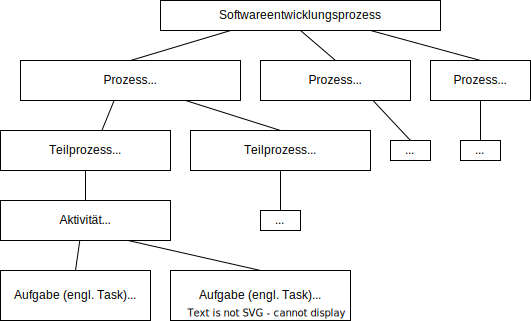
\includegraphics[scale=1.0]{Bilder/Kapitel-1/Abb-1-6.pdf}
	\caption{Zusammenhang zwischen Prozessen, Aktivitäten und Aufgaben}
	\label{fig:prozesse_aktivitaeten_aufgaben}
\end{figure}

Abbildung~\ref{fig:prozesse_aktivitaeten_aufgaben} zeigt den Zusammenhang \marginline{Prozess, Aktivität, Aufgabe} der in diesem Text verwendeten Begriffe: Ein Prozess, wie zum Beispiel der Prozess der Anforderungsermittlung, kann in \mbox{\textit{Teilprozesse}} weiter unterteilt werden. Jeder Teilprozess besteht aus einer Menge von \textit{Aktivitäten}, wie zum Beispiel „Lastenheft erstellen“ oder „Module der Software bestimmen“. Aktivitäten wiederum können in noch kleinere Einheiten, sogenannte \textit{Aufgaben} (engl. Tasks), unterteilt werden, die schlussendlich von Rollen ausgeführt werden. Ein konkreter Softwareentwicklungsprozess ist somit eine Menge aus einzelnen Aktivitäten zusammengesetzter Prozesse. Dabei können sich die Prozesse oder Teilprozesse auch überschneiden, sodass es häufig nicht möglich ist genau zu bestimmen, an welcher Stelle ein Prozess bzw. Teilprozess endet und ein anderer beginnt. Ebenso lässt sich nicht immer eindeutig bestimmen, welchem Teilprozess eine konkrete Aufgabe zugeordnet ist. 

Der Software Engineering Body of Knowledge (SWEBOK) definiert einen ingenieurwissenschaftlichen Prozess als

\sttpzitat{„a set of interrelated activities that transform one or more inputs into outputs while consuming resources to accomplish the transformation“. \cite[8-1]{swe14}}{}

Bezogen auf den Gesamtprozess der Entwicklung eines Softwareprodukts besteht der Input aus der Menge der Anforderungen an die zu erstellende Software und der Output aus dem fertigen Softwareprodukt. Die einzelnen Prozesse innerhalb des Softwareentwicklungsprozesses transformieren unterschiedliche Arten von Inputs in Outputs, wobei die Outputs eines Prozesses oft die Inputs eines oder mehrerer Folgeprozesse sind. So könnte zum Beispiel der Output eines Implementierungsprozesses ein Stück Programmcode sein und Letzteres ein Teil des Inputs für den Prozess des Testens. Bei den verbrauchten Ressourcen für die Erstellung des Softwareprodukts handelt es sich in erster Linie um die Arbeitszeit der an der Entwicklung beteiligten Personen. Ressourcen können aber zusätzlich auch Softwareressourcen (\zb fertige Softwarekomponenten, die in das Produkt eingebunden werden, oder für die Entwicklung verwendete Tools) und Hardwareressourcen (\zb Entwicklungsinfrastruktur) sein. 

\sttpHinweiskasten{1.0}{unterschiedliche Begriffsverwendung}{Beachten Sie, dass Teile der Literatur die großen Bereiche des Software\-entwicklungsprozesses wie Anforderungsermittlung/-analyse, Implementierung oder Testen nicht als \textbf{Prozesse}, sondern schon als \textbf{Aktivitäten} bezeichnen. Für konkrete Tätigkeiten, wie zum Beispiel für die Tätigkeit „das Lastenheft erstellen“ innerhalb der Anforderungs\-ermitt\-lung/-analyse werden dann Begriffe wie Unteraktivitäten oder Sub-Aktivitäten verwendet.}

Bei den angesprochenen Prozessen 
\marginline{Kernprozesse, unterstützende Prozesse}
des Softwareengineering unterscheidet man \textit{Kernprozesse} (engl. primary processes, development processes, implementation processes) von \textit{unterstützenden Prozessen} (engl. support processes). Letztere werden häufig auch als Softwaremanagementprozesse bezeichnet. Seit Mitte der 1980er Jahre besteht relative Einigkeit darüber, welche \textbf{Kernprozesse} dem Softwareengineering zuzurechnen sind, auch wenn die Benennungen, die konkreten Aktivitäten und die Abgrenzungen zwischen den Prozessen je nach Blickwinkel differieren können. Die Kernprozesse des Softwareengineering sind:
\begin{itemize}
	\item die Anforderungsermittlung/-analyse
	\item der Softwareentwurf
	\item die Implementierung
	\item das Testen bzw. allgemeiner die Qualitätssicherung sowie
	\item die Wartung, ggf. ergänzt um die Weiterentwicklung der Software
\end{itemize}

Mittlerweile ist unbestritten, dass neben den Kernprozessen auch Softwaremanagementprozesse Teil des Softwareengineering sind. Welche Managementprozesse dies genau betrifft, variiert aber stark in der Literatur. Der Schwerpunkt unserer Lehrveranstaltung liegt auf den Kernprozessen des Softwareengineering. 

\minisec{Aufbau des Textes}

Lassen Sie uns an dieser Stelle die inhaltliche Ebene kurz verlassen und auf die noch ausstehende Darstellung zum Aufbau des Textes zurückkommen. Kapitel~\ref{sec:Kap-2} in dieser ersten Lektion behandelt das Thema der Vorgehensmodelle und deren Zusammenhang zu den Prozessen des Softwareengineering. Die detaillierte Beschäftigung mit den eben vorgestellten Kernprozessen des Softwareengineering beginnt ab Lektion 4. Zuvor werden sich die Lektionen 2 und 3 allgemeiner mit dem Thema Modellierung beschäftigen, das in allen Prozessen des Softwareengineering eine Rolle spielt. Wie erwähnt legt der Text den Schwerpunkt auf grundlegende Aspekte des Softwareengineering, die weitestgehend unabhängig von der Art des (zu entwickelnden) Softwareprodukts sind. Einige andere Einschränkungen müssen wir aber treffen, um den Umfang im Rahmen zu halten: Die Lehrveranstaltung beschäftigt sich nur mit objektorientierter Softwareentwicklung und aus der Menge der möglichen Notationssprachen wird die Unified Modeling Language (UML) gewählt, die die bei Weitem größte Verbreitung genießt.  